\subsection{Optimizers}


Training a large deep neural network is very computationally expensive. The training of CNN and LSTM are typically optimized using Stochastic Gradient (SG) and Adam based methods.  At each step $t$ a minibatch of $B$ samples $x_i$
is selected from the training set. Increasing the capacity of the mini-batch permits scaling to more nodes without reducing
the workload on each unit. At the same time, training with a large batch has been observed to be difficult \cite{Krizhevsky}. Krizhevsky (2014) suggested the following rules for training with large batches: when you increase
the batch $B$ by $k$, you should also increase the learning rate by $k$ in order to do reduce $k$ steps.  It was observed that linear scaling works much better for networks with Batch
Normalization (e.g. Codreanu et al. (2017)). For example Chen et al. (2016) trained the Inception
model with batch $B=6400$, and Li (2017) trained Resnet-152 for $B=5K$. Two main problems of such large batch training include: 

\begin{itemize}
    \item The instability of training with high learning rates (LR). Goyal et al. suggested the LR warm-up policy to start with a small LR and switch to the regular LR after a few epochs. They were able to combine that with linear scaling to train Resnet-50 with batch $B=8K$ with loss in accuracy. 
    
    \item There is a lack of generalization ability, according to Keskar et al. \cite{Keskar}, the large-batch methods seem to converge to sharp minimizers of the training function. Adaptive learning rates have gathered interests to solve this problem and also to help reduce the hand-tuning of hyperparameters \cite{}.  
\end{itemize}




You et al. (2017) proposed a new training algorithm of LARS to solve this problem. The intuition is to adapt the learning rate on each layers that is SG based. Using the LARS algorithm, the Alexnet can be trained with a batch size of 8k and Resnet-50 can be trained with a batch size of 32k without loss in accuracy. However, LARS performs poorly for attention models like BERT. 


Inspired by LARS, You et al. (2019) developed a new optimization algorithm Layer-wise Adaptive Moments optimizer for Batch training (LAMB) especially for large batch size training. The adaptivity of LAMB are different from LARS in two parts: (1) parameter normalization based on the square root of the second moment in Adam; and (2) layer-wise adaptive normalization. The author reported that by training the BERT language model with LAMB optimizer can drastically reduce the training time from 3 days to 76 minutes without the reduction of performance.

\subsection{Case Studies}


\subsubsection{Computer Vision - Image Classification}

\begin{figure}[!t]
    \centering
    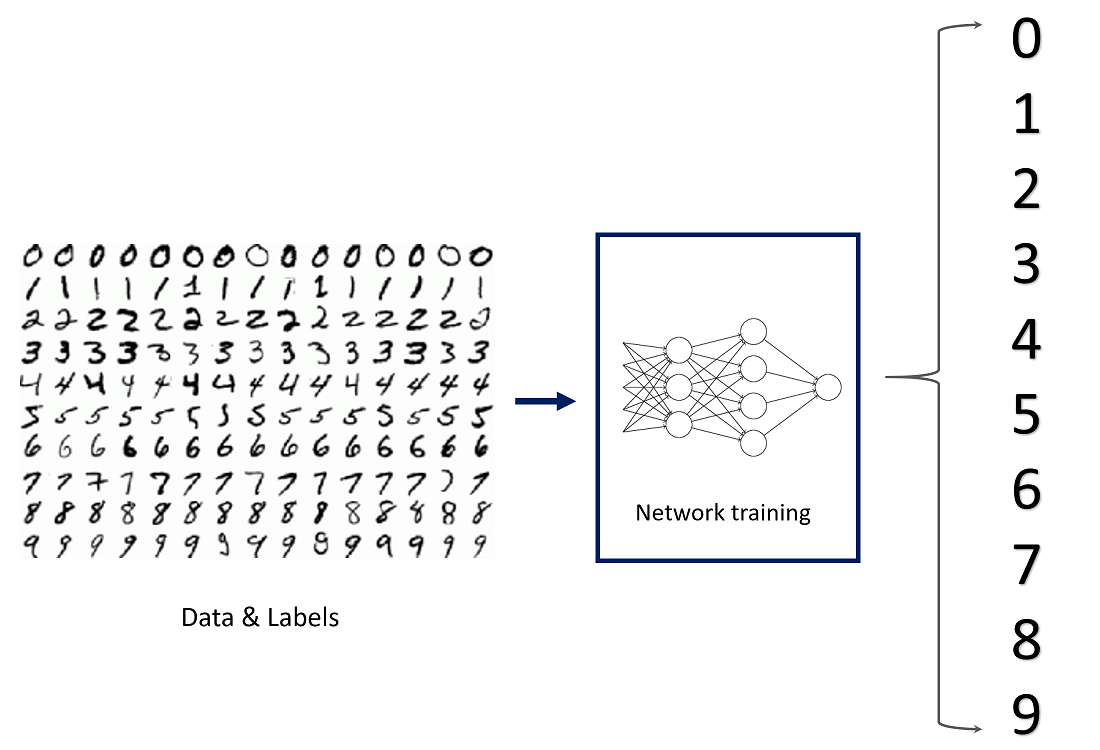
\includegraphics[width=\linewidth, height=7cm]{img/mnist.png}
    \caption{An overview of the image classification in an example of handwritten digits classification.}
    \label{fig:DrQA_overview}
    \vspace{-10pt}
\end{figure}

One of the classical task over the past 10 years in the machine learning community is image classification with the proposal of many new models and the creation of benchmark datasets. For instance, this study focuses on handwritten digit recognition or optimal character recognition (OCR) of MNIST database by LeCun et al. \cite{LeCun}. Before the advancement of GPU is 2012, traditional machine learning approaches have served as the baseline for this OCR task tested on MNIST database including K-Nearest Neighbor, ensemble-based classifiers, and Support Vector Machine. After 2012, Convolutional Neural Network (CNN) emerged and served as the new baseline for this benchmark dataset in OCR task.
The traditional CNN model, where the earliest date can be traced back
to the 1986 Back Propagation algorithm \cite{BP}. Then in 1989 LeCun used it
in multi-layer neural networks \cite{1989Lecun} which is then extended to LeNet-5 model in 1998. The CNN's architecture allows take advantage of the
two dimensional structure of the input data in order to capture a deeper understanding of these images.



\begin{figure}[!t]
    \centering
    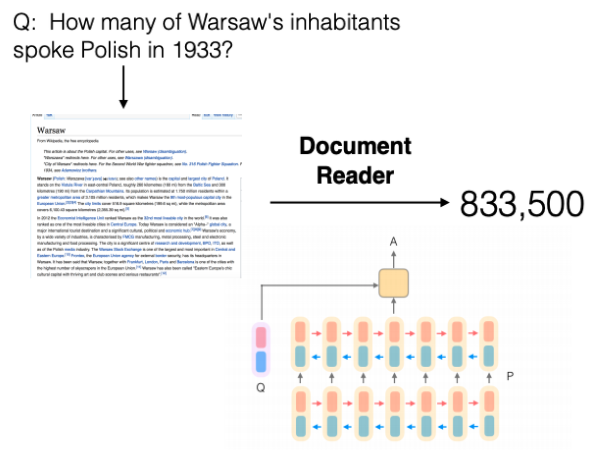
\includegraphics[width=\linewidth]{img/QA.png}
    \caption{An overview of the question answering system DrQA \cite{}.}
    \label{fig:DrQA_overview}
    \vspace{-10pt}
\end{figure}



\subsubsection{NLP - Question Answering System}

The NLP specific task we picked for this paper is open-domain QA originally rooted in finding answers in collections of unstructured documents following the annual Text REtrieval Conference competitions (TREC\footnote{https://trec.nist.gov/data/qamain.html}). First, the development of Knowledge Base (KBs) have pushed a lot of resources creation like WebQuestion \cite{webquestion} and SimpleQuestion \cite{simplequestion} or automated extracted KBs like NELL \cite{KBNELL}. Yet, KBs have inherent nature that limiting these work including fixed schemas and incompleteness. Therefore, researchers have to return to the original setting of answering from raw text. 



Secondly, it is a distinct subfield of machine comprehension of text. With the advancement of deep learning architectures like attention-based and memory-augmented neural network \cite{}, researchers have made considerable progress.  The QA system adopted for this study shall utilize these new methods.


Other previous researchers also considered other resources of semi-structured knowledge such as infoboxes, article structure, category structure, and definitions \cite{}. Yet, this QA system only consider the comprehension of text only, or relying on a single resource.
    
    






Therefore, this study focused on the inspired Document retriever Question Answering (DrQA) similar to Figure \ref{fig:DrQA_overview}. As the name suggested, it composed of (1) Document Retriever and (2) Document Reader where for this study's purpose of model's optimization will not consider part 1 of the system and solely focus on part 2. Specifically, for Document
Reader, a multi-layer recurrent neural network
machine comprehension model trained to detect
answer spans in those defined context.




\subsubsection{Speech - Speech-to-Text}

Another study case which is essential to a lot of virtual or smart home assistant is speech recognition. As previously mentioned, our goal is to output reasonable transcription according to the audio segment. A general system is illustrated in the Figure \ref{fig:speech2text}. For more than 20 years ago, feed-forward
neural network acoustic models were explored \cite{}.  More recently DNNs have become a fixture in the ASR pipeline with almost all
state of the art speech work containing some form of deep neural network \cite{}. From CNN successes with acoustic models \cite{}, recurrent
neural networks (typically LSTMs), are beginning to be adapted in state-of-the art recognizers \cite{} that thrive on convolutional layers for the feature extraction \cite{}. World-wide recognized level of such models include Deep Speech by Baidu \cite{} and Listen Attend Spell (LAS) by Google \cite{}. We adapted a model that is similar to Deep Speech 2 architecture \cite{} which utilized enhanced numerical optimization through SortaGrad and Batch normalization, RNNs evaluation with larger strides with bigram outputs, and searching through bidirectional and unidirectional models.


\begin{figure}[!t]
    \centering
    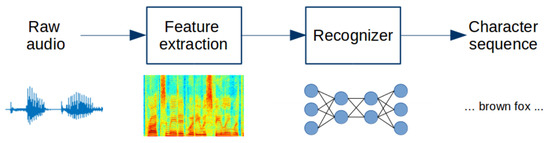
\includegraphics[width=\linewidth]{img/speech2text.jpg}
    \caption{An overview of Speech 2 Text end to end system}
    \label{fig:speech2text}
\end{figure}

For learning the audio features, the author employed the Residual CNN which was first introduced by He et al. \cite{} to learn the skip connections (i.e. residual connections) for faster and more generalizable audio features. Specifically, these networks shall have a smoother loss surface when visualizing to make it easier to navigate the landscape and find a lower and more generalizable loss minima.  For leveraging the previously learned features, the bidirectional recurrent neural network (RNN) is employed which first introduced by for being good at sequence modeling problem. Specifically, RNN helps learn the context of frame before each step and the frame after it as well. The author employed Gated Recurrent Unit (GRU's) variant which is simpler than traditional Long Short Term Memory (LSTM) in (1) avoiding the usage of memory unit that LSTM does and (2)  LSTMs have computations  separating the update gate and forget gate which lead to the architecture more complex and less efficient to GRU. 


